\documentclass[dvipdfmx,11pt,notheorems]{beamer}
\usepackage{slide}

\setkeys{slide}{footer={Division of Informatics, Graduate School of Informatics, Kyoto University}}

\title{Example: Slide style}
\author{OKAMOTO Yuta}
\institute{Division of Informatics, Graduate School of Informatics, Kyoto University}
\date{\today}

\begin{document}

\begin{frame}
  \titlepage
\end{frame}

\begin{frame}
  \framesection{Mathematical}
  Let $\left( C, \partial \right)$ be a chain complex, define the $k$-cycle $Z_k$ and $k$-boundary of $\left( C, \partial \right)$ by
  \begin{align*}
    Z_k = \mathrm{Ker}\ \partial_k,\ B_k = \mathrm{Im}\ \partial_k.
  \end{align*}
  Then, we can define the $k$-th homology of $\left( C, \partial \right)$ as following definition.
  \begin{dfn}
    The $k$-th homology $H_k$ of the chain complex $\left( C, \partial \right)$ is defined by the quote module
    \begin{align*}
      H_k = Z_k / B_k.
    \end{align*}
  \end{dfn}
\end{frame}

\begin{frame}[containsverbatim]
  \framesection{Code block}

  Bachelor's degree. Department of Mathematics, Faculty of Science, University of Tokyo : 2020 April - 2024 March.

  \lstinputlisting[language=python]{example.py}
\end{frame}

\begin{frame}
  \framesection{Two column}
  \begin{columns}[c]
    \begin{column}{0.6\textwidth}
      During my undergraduate years, I majored in mathematical physics. Specifically, I focused on formulating quantum mechanics using operators on Hilbert spaces, based on John von Neumann's ``Mathematical Foundations of Quantum Mechanics.''
    \end{column}
    \begin{column}{0.4\textwidth}
      \begin{center}
        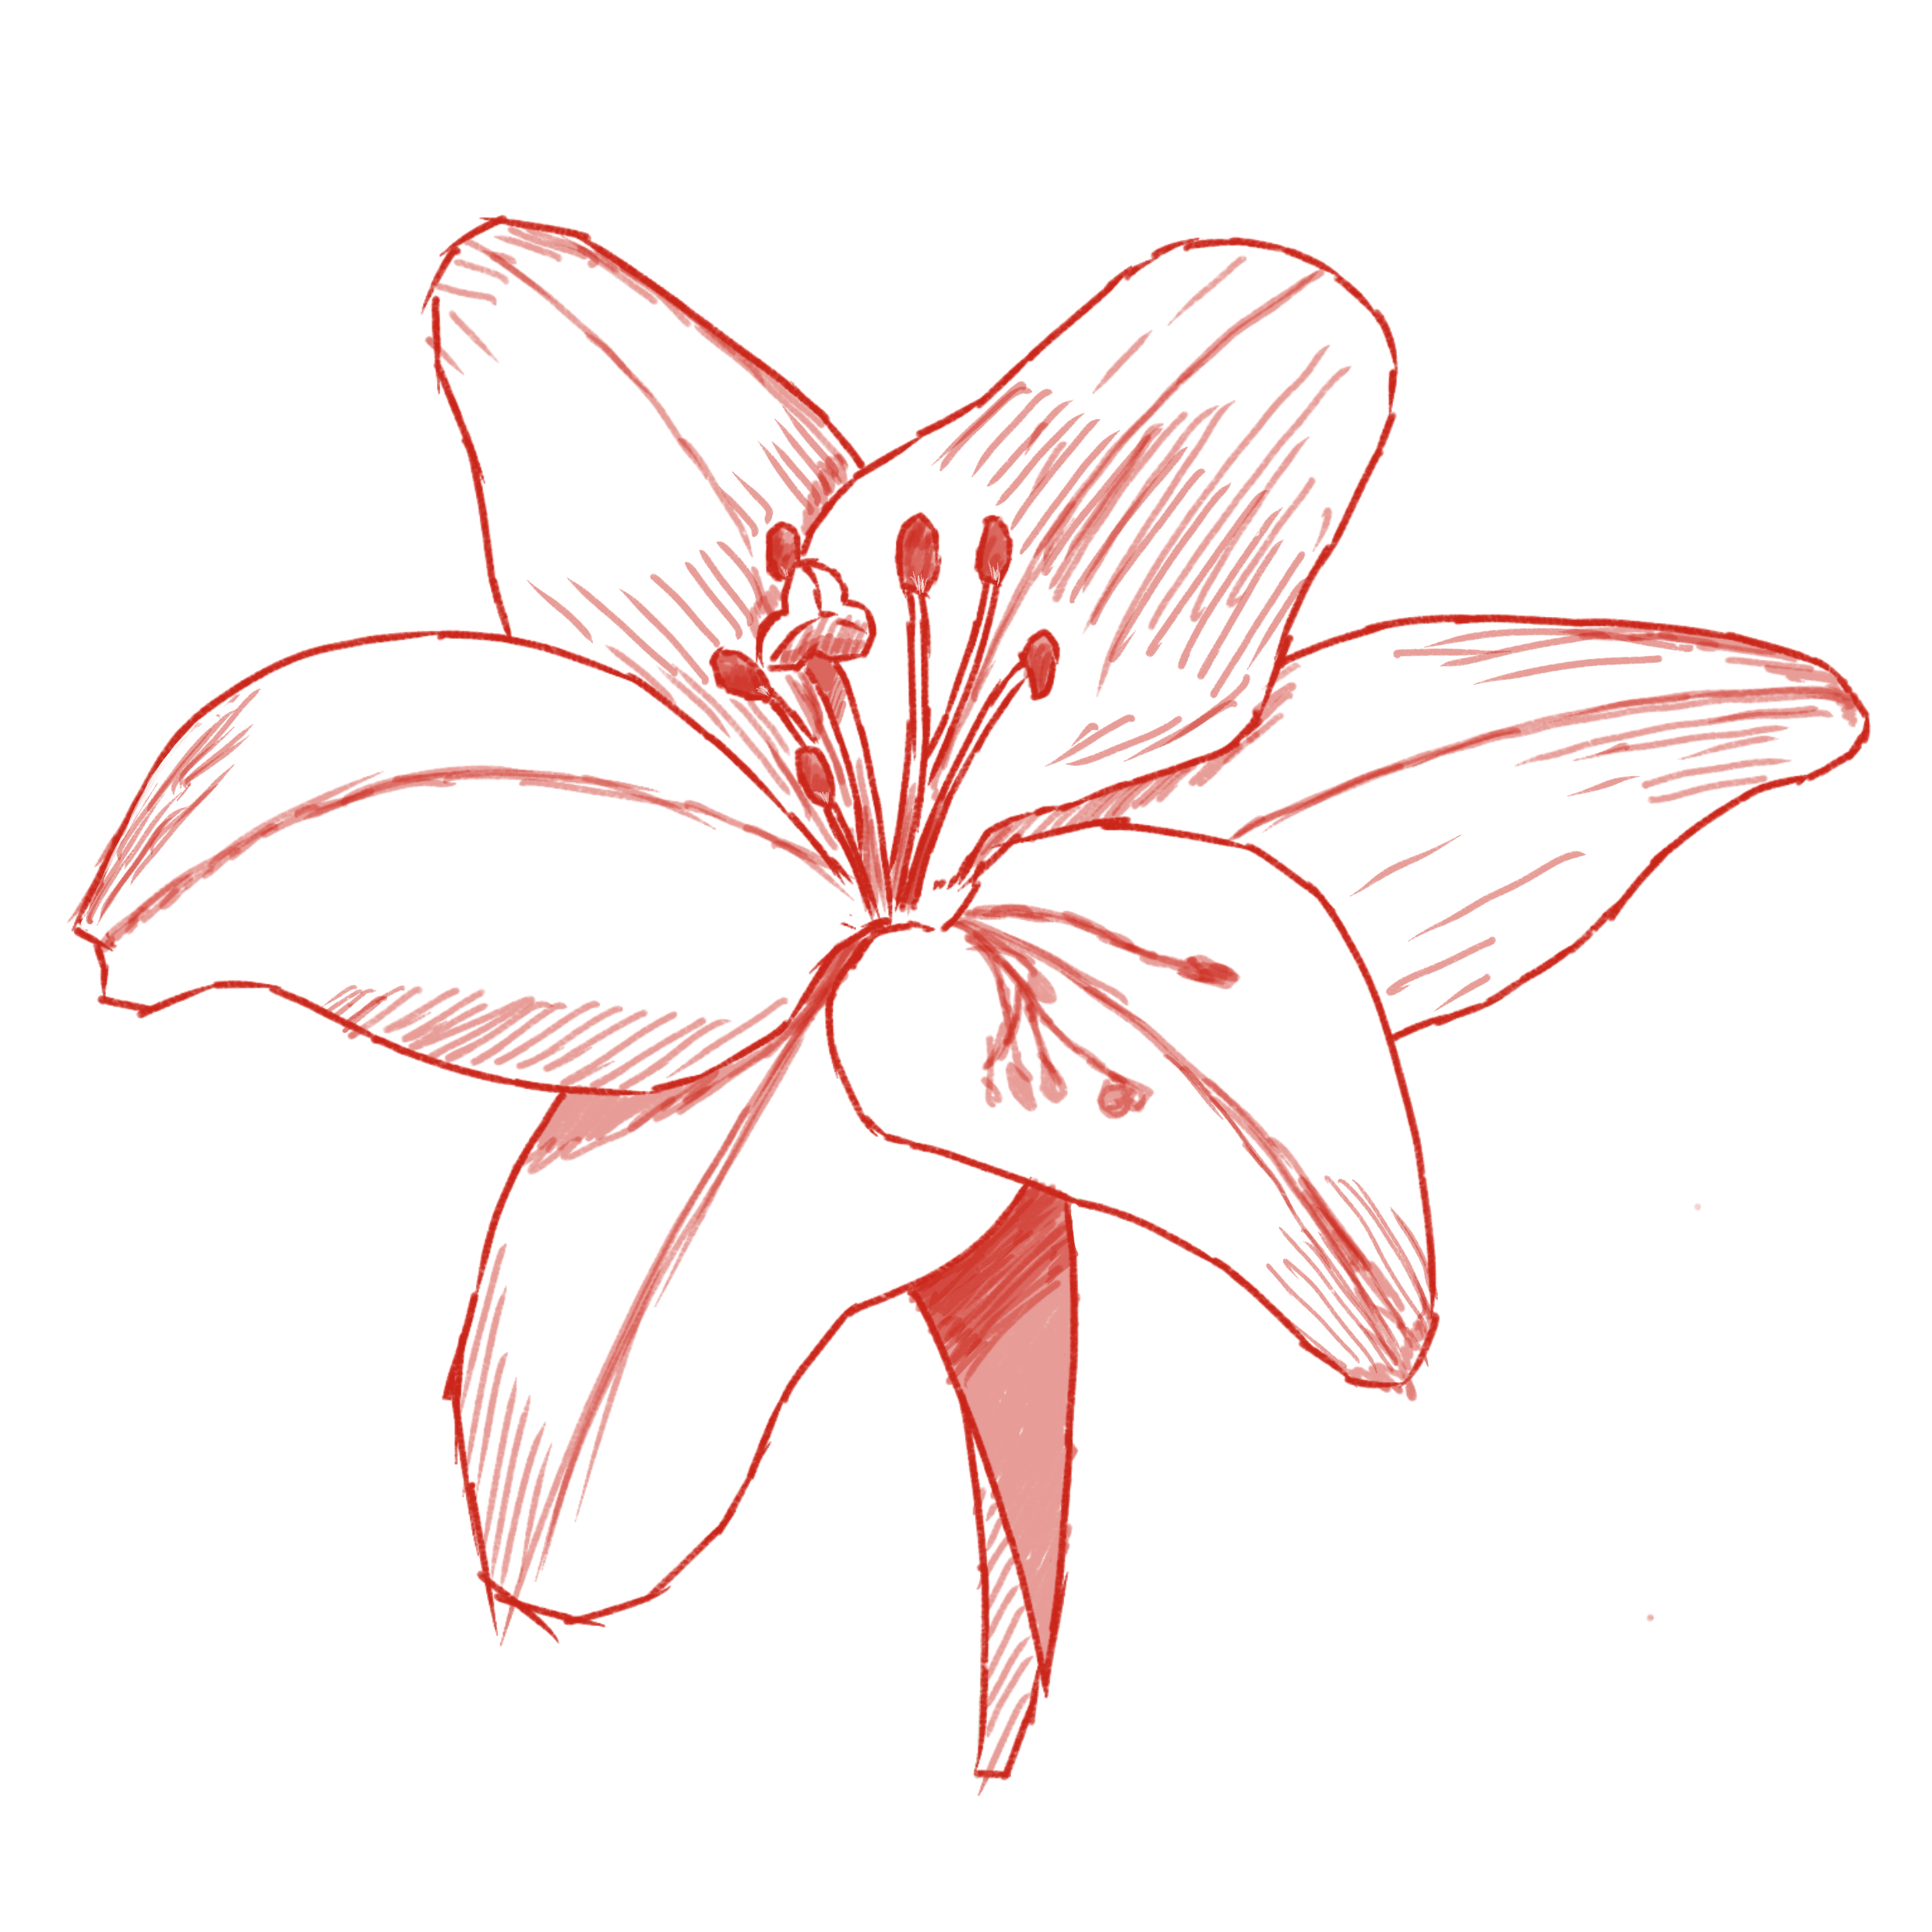
\includegraphics[width=0.8\columnwidth]{global_okmtyuta.png}
      \end{center}
    \end{column}
  \end{columns}
\end{frame}

\end{document}